\documentclass{article}
\usepackage[utf8]{inputenc}
\usepackage{graphicx}
\usepackage{enumitem}

\begin{document}
\begin{titlepage}
    \centering
    {\scshape\large AY 2022/2023 \par}
    \vfill
    
\includegraphics[width=100pt]{logo-polimi-new.pdf}
    \par\vspace{1cm}
    {\scshape\LARGE Politecnico di Milano \par}
    \vspace{1.5cm}
    {\huge\bfseries Green Home B\par}
    {\Large {Advanced User Interfaces}\par}
    \vfill
    {\large Professor\par Franca \textsc{Garzotto}}
    \vspace{2cm}
      \vfill
    {\huge {\textbf{Design and Technology}}\par}
      \vfill
    {\Large {Ottavia Belotti\quad Alessio Braccini\quad\quad\quad\quad\quad\quad\quad\quad Francesco Dubini \quad Hanyu Zhu}\par}
    
\end{titlepage}

\pagenumbering{gobble}
\begin{abstract}
    abstract TODO
\end{abstract}
\newpage
{\huge{The team}}\\

    \begin{tabular}{ll}
    
        
\includegraphics[width=100pt]{Coco.png} & \vspace{-50px}
        \begin{tabular}{l}        
            \textbf{Name}: Ottavia belotti\\
            \textbf{Email}: ottavia.belotti@mail.polimi.it\\
            \textbf{Phone} Number: ????\\
            \textbf{Master Program}: Computer Science and Engineering\\ \vspace{100px}
        \end{tabular}\\

        
\includegraphics[width=100pt]{Ale.png} & \vspace{-50px}
        \begin{tabular}{l}
            \textbf{Name}: Alessio Braccini\\
            \textbf{Email}: alessio.braccini@mail.polimi.it\\
            \textbf{Phone} Number: ????\\
            \textbf{Master Program}: Computer Science and Engineering\\ \vspace{100px}
        \end{tabular}\\

        
\includegraphics[width=100pt]{Dubs.png} & \vspace{-50px}
        \begin{tabular}{l}
            \textbf{Name}: Francesco Dubini\\
            \textbf{Email}: franceso.dubini@mail.polimi.it\\
            \textbf{Phone} Number: ????\\
            \textbf{Master Program}: Computer Science and Engineering\\ \vspace{100px}
        \end{tabular}\\

        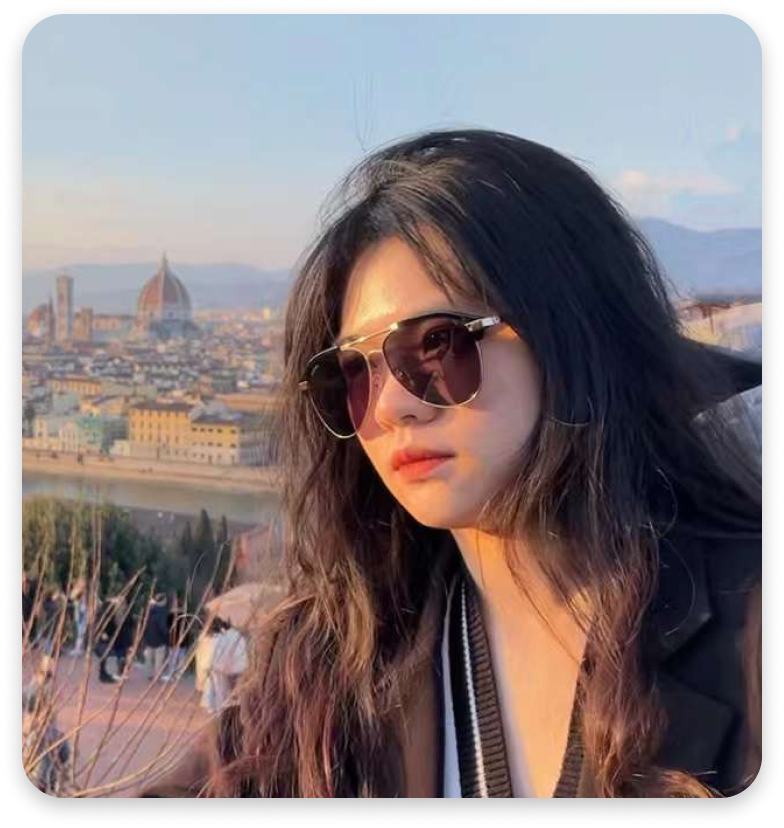
\includegraphics[width=100pt]{Hanyu.png} &  \vspace{-100px}
        \begin{tabular}{l}
            \textbf{Name}: Hanyu Zhu\\
            \textbf{Email}: hanyu1.zhu@mail.polimi.it\\ 
            \textbf{Phone} Number: ????\\
            \textbf{Master Program}: Desing stuff HANYU PLEASE CORRECT IT \\ \vspace{100px}
        \end{tabular}\\
    \end{tabular}

    
\newpage
\pagenumbering{roman}
\tableofcontents
\newpage
\pagenumbering{arabic}

\section{Executive Summary}
    cose
\newpage

\section{Introduction}

\newpage

\section{Requirements}
    \subsection{Main Target Groups}
    Before pointing out goals, target groups and requirements of our project is useful to consider which stakeholders are involved:
        \begin{itemize}
            \item House owner
            \item Energy aware people
            \item Climate change concerned people
            \item Edison researchers
        \end{itemize}
    \subsection{Context and Needs}
        The context of our project is a smart mirror with a vocal assistant that helps you in energy saving % where such needs emerge (and where your solution will be used)

        %Please notice that NEEDS are properties of the stakeholders/end users, while GOALS are properties of your technological system, i.e., describe what you want to achieve, but not HOW
        % (“how” is described in the UX design section and, al a lower level of abstraction, in the
        % Implementation section). Goals are at a lower level of abstraction than Needs and more
        % concrete/specific. 
        

        The needs are:
        \begin{itemize}
            \item[N1] Save on energy related costs
            \item[N2] Acquire energy consumption and production data
            \item[N3] Reduce waste of energy
            \item[N4] Study costumers'habits
            \item[N5] Provide to users energy saving related functionalities
        \end{itemize}
    \subsection{Goals}
        \begin{itemize}
            \item[G1] Inform user about energy consumption/production in accessible and intuitive way
            \item[G2] Give feedback on most energy efficient ways to use home devices
        \end{itemize}
    \subsection{Constraints}
        \begin{itemize}
            \item[C1] Mirror dimensions and components equipment (microphone, speaker, touchscreen)
            \item[C2] Data sources: smart plugs, smart devices
            \item[C3] Limited amount of time the user spend in front of the mirror
        \end{itemize}
\newpage   

\section{State of the Art ???}
\newpage   
   
\section{Solution - UX Design}
    \subsection{General Approach}
    \subsection{Interaction and Interfaces}
    \subsection{Scenarios}

    %     - Suggestion for conversational interaction projects: include (examples of) dialogue diagrams that highlight how the conversation unfolds

\newpage  

\section{Solution - Implementation}
    \subsection{Hardware}
    
    \subsection{Software}
\newpage   

\section{Empirical Evaluation}Forse possiamo non farla
    \subsection{Focus}
    \subsection{Research Goal}
    \subsection{Participants}
    \subsection{Procedure}
\newpage   

\section{Value proposition/Onliness statement}
% Concisely formulate which value you promise to your users/customers and what makes your
% “product” special or unique for them
% - Why is this a «good» solution?
% - Are there competitors? If yes, why is your solution better than the existing ones?
\newpage   

\section{Future Works}
    %     - A critical reflection on your work (challenges, critical aspects, main difficulties
    % encountered…) and on the real potential of the technology you have developed to address
    % the needs of your target group and maybe of other targets…
    % - What was left out and future directions (what could be done next in the short - medium
    % term, visions in the long term…)
\newpage   

\section{Member contribution}
    Member Contribution (IMPORTANT!): a table where you declare the main role and contribution
    that each group member has provided to the project; the table has the following structure:
    Member-Name-Surname; Main Role/Contribution. Role/Contribution is described in 2-3 lines
\newpage   

\section{Bibliography ???}
\newpage   

\end{document}
